% !TEX root = ../sparsity_thesis.tex
\chapter{Introduction}
\label{ch:introduction}

\section{Background}
\label{sec:background}

Enterprise Resource Planning (ERP) systems have evolved over the past two decades from monolithic, on-premise installations affordable only to large corporations into cloud-delivered, multi-tenant Software-as-a-Service (SaaS) platforms accessible to small and medium-sized enterprises (SMEs). This democratization has been driven by the multi-tenant architectural model, in which a single application instance---or a single application instance coupled with isolated per-tenant databases---serves many customer organizations simultaneously, dramatically reducing the marginal cost of onboarding a new business. As a consequence, the modern ERP is no longer merely a transactional system of record for finance, sales, and human resources; it is increasingly expected to function as an analytical platform capable of forecasting late payments, scoring sales leads, and predicting employee attrition.

The mechanism through which contemporary ERP vendors deliver these analytical capabilities is machine learning (ML). Tabular classifiers such as gradient-boosted decision trees and random forests have proven highly effective at predicting business outcomes from the structured operational data that ERPs accumulate. However, these models are widely characterized as ``black boxes'': their internal decision logic is not directly interpretable by the business users who are expected to act on their outputs. In a B2B context where an algorithmic recommendation may directly influence whether credit is extended to a customer, whether a salesperson pursues a lead, or whether a manager intervenes to retain an employee, an opaque prediction is operationally unacceptable and, under emerging regulation such as the European Union's Artificial Intelligence Act, increasingly legally untenable.

The academic and industrial response to this opacity has been the rapid maturation of the field of Explainable Artificial Intelligence (XAI). Post-hoc, model-agnostic techniques---most prominently SHapley Additive exPlanations (SHAP) and Local Interpretable Model-agnostic Explanations (LIME)---have emerged as de facto standards for translating the predictions of any tabular classifier into human-readable feature attributions. The prevailing narrative in both the literature and vendor marketing positions SHAP and LIME as the architectural component that closes the loop between predictive ML and trustworthy business decision-making.

This narrative, however, has been validated almost exclusively on data-rich settings: large, mature, single-tenant enterprises whose historical record contains tens of thousands of labelled transactions. The multi-tenant SaaS ERP context is fundamentally different. In a platform serving thousands of tenants, the data volume per tenant follows a long-tail distribution: a small number of mature customers contribute the bulk of the records, while the majority of tenants---particularly newly-onboarded SMEs---operate in a persistent state of data scarcity, the so-called \emph{cold-start} regime. Under such conditions, a per-tenant ML model is trained on a handful of observations and consequently exhibits little to no genuine predictive power.

What has gone largely unexamined in the literature is the behaviour of post-hoc XAI techniques under exactly these conditions. SHAP and LIME are \emph{unconditional} explainers: they will produce a confidently-rendered, visually-compelling attribution diagram for any prediction made by any model, regardless of whether that model is actually learning a signal or merely interpolating noise. The result is a phenomenon this thesis names the \textbf{hallucinated explanation}: a polished, business-grade narrative (``This invoice is at risk of late payment primarily because of \texttt{payment\_value} and \texttt{freight\_value}'') that is generated with full visual authority on top of a model whose discriminative performance is statistically indistinguishable from random guessing. For the cold-start SME tenant, the XAI layer that was supposed to function as a trust-building safeguard becomes, instead, a mechanism for the systematic manufacture of false confidence.

\begin{figure}[h]
    \centering
    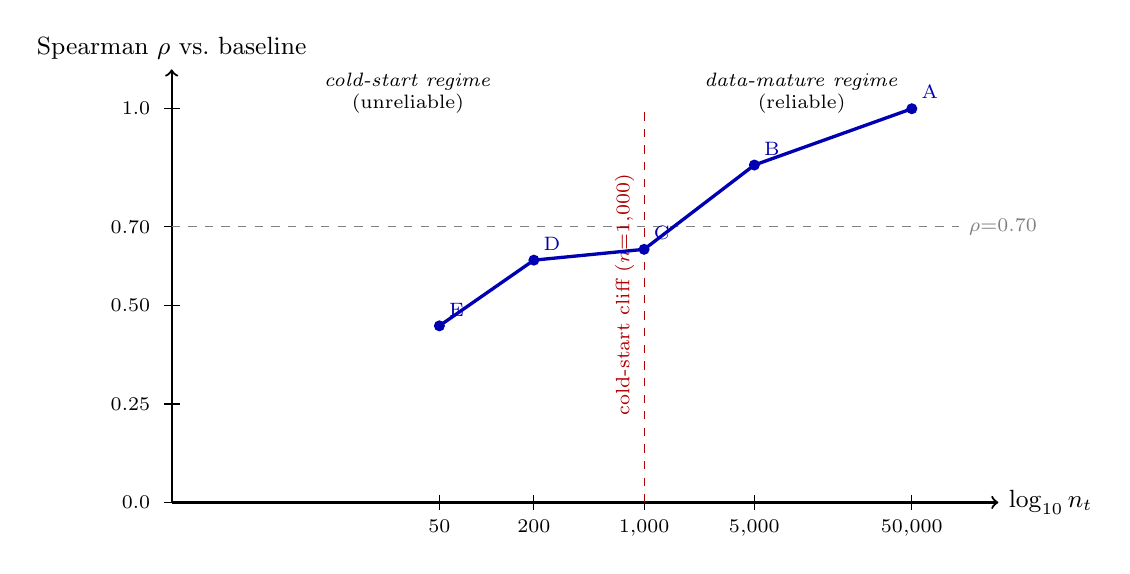
\begin{tikzpicture}[x=1.0cm,y=1.0cm]
        % Axes
        \draw[->,thick] (0,0) -- (10.5,0) node[right] {\small $\log_{10} n_t$};
        \draw[->,thick] (0,0) -- (0,5.5) node[above] {\small Spearman $\rho$ vs.\ baseline};
        % y-axis ticks
        \foreach \y/\lab in {0/0.0, 1.25/0.25, 2.5/0.50, 3.5/0.70, 5/1.0} {
            \draw (-0.1,\y) -- (0.1,\y);
            \node[left,font=\scriptsize] at (-0.15,\y) {\lab};
        }
        % x-axis ticks at tenant tiers: log10(50)=1.7, log10(200)=2.3, log10(1000)=3, log10(5000)=3.7, log10(50000)=4.7
        \foreach \x/\lab in {1.7/{50}, 2.3/{200}, 3/{1{,}000}, 3.7/{5{,}000}, 4.7/{50{,}000}} {
            \draw (\x*2,-0.1) -- (\x*2,0.1);
            \node[below,font=\scriptsize] at (\x*2,-0.1) {$\lab$};
        }
        % Reliability threshold rho = 0.70
        \draw[dashed,gray] (0,3.5) -- (10,3.5);
        \node[gray,font=\scriptsize,right] at (10,3.5) {$\rho{=}0.70$};
        % Cold-start cliff vertical at n=1000 (x = 3*2 = 6)
        \draw[dashed,red!70!black] (6,0) -- (6,5);
        \node[red!70!black,font=\scriptsize,above,rotate=90] at (6,2.5) {\quad cold-start cliff ($n{=}1{,}000$)};
        % Empirical curve through (1.7,2.24)=E, (2.3,3.08)=D, (3,3.21)=C, (3.7,4.28)=B, (4.7,5)=A
        % rho: A=1.00, B=0.857, C=0.6429, D=0.6154, E=0.4485 -> y = rho*5
        \draw[very thick,blue!70!black,line cap=round]
            (1.7*2,0.4485*5) -- (2.3*2,0.6154*5) -- (3*2,0.6429*5) -- (3.7*2,0.857*5) -- (4.7*2,1.0*5);
        \foreach \x/\y/\lab in {1.7/{0.4485}/E, 2.3/{0.6154}/D, 3/{0.6429}/C, 3.7/{0.857}/B, 4.7/{1.0}/A} {
            \fill[blue!70!black] (\x*2,\y*5) circle (2pt);
            \node[above right,font=\scriptsize,blue!70!black] at (\x*2,\y*5) {\lab};
        }
        % Regime labels
        \node[font=\scriptsize,align=center] at (3,5.2) {\textit{cold-start regime}\\(unreliable)};
        \node[font=\scriptsize,align=center] at (8,5.2) {\textit{data-mature regime}\\(reliable)};
    \end{tikzpicture}
    \caption{The ``Reliability Cliff'' in multi-tenant XAI. Spearman rank
    agreement of per-tenant SHAP rankings against the data-rich reference
    (Tenant~A) plotted against tenant size $n_t$ on a logarithmic axis.
    Agreement collapses below the conventional $\rho = 0.70$ reliability
    threshold at the $n = 1{,}000$ tier (Tenant~C), marking the operational
    cold-start boundary used by the Maturity-Aware Routing gate. Values
    plotted are the leakage-corrected empirical figures from Chapter~\ref{ch:results}.}
    \label{fig:reliability_cliff_concept}
\end{figure}

Preliminary empirical work conducted as part of this study quantifies this phenomenon for the first time in a multi-tenant ERP setting. Using the Olist Brazilian e-commerce corpus partitioned into five synthetic tenants of decreasing size (50{,}000; 5{,}000; 1{,}000; 200; and 50 records), and under a strict leakage-avoidance regime in which only order-time observables are admitted into the feature matrix, the Spearman rank correlation between local SHAP attributions and the data-rich baseline was observed to fall monotonically from $1.000$ to $0.449$, and the absolute SHAP variance simultaneously rose by more than two orders of magnitude---from $0.022$ at the data-rich tier to $5.04$ at the cold-start tier. By contrast, classical predictive metrics offered no warning of this regime change: AUC-ROC remained uniformly modest (between $0.61$ and $0.66$) across the data-rich, medium, sparse, and very-sparse tiers, and \emph{rose} anomalously to $0.89$ at the cold-start tier as a small-sample artefact. These figures motivate the central claim of this thesis: in multi-tenant ERPs, XAI cannot be deployed as a uniform, tenant-agnostic feature; it must be governed by an architectural mechanism that is aware of each tenant's data maturity \emph{and that monitors explanation-fidelity metrics directly}, because predictive metrics alone cannot localise the cold-start cliff.

\section{Problem Statement}
\label{sec:problem-statement}

The problem addressed by this research arises at the intersection of three structurally interconnected issues that, taken together, render the na\"ive deployment of XAI in multi-tenant ERPs unsafe.

\paragraph{Problem 1 --- Cold-start data sparsity in multi-tenant ERPs.}
The multi-tenant SaaS model, by design, exposes the platform to a wide spectrum of customer maturity levels. A newly-onboarded SME tenant may possess only tens or low hundreds of invoices, leads, or employee records at the moment when the ML and XAI capabilities of the platform are first activated for them. Per-tenant ML models trained on such cohorts cannot, in general, recover the underlying statistical structure of the business process they are meant to predict, and consequently degrade towards random performance.

\paragraph{Problem 2 --- The ``hallucinated explanation'' phenomenon.}
Post-hoc explainers such as SHAP and LIME continue to produce confident, well-formatted attribution outputs even when the underlying model is no longer predictive. The empirical evidence developed in this study makes this concrete: at the $n = 1{,}000$ tier, Spearman fidelity has already fallen to $0.6429$, which is below the $0.70$ reliability threshold conventionally used in the explanation-stability literature; at $n = 200$, the absolute SHAP variance reaches $0.2017$, an order of magnitude above the data-rich baseline of $0.0224$, indicating an unstable attribution surface; and at $n = 50$, the explanations are still rendered to the end user even though the underlying model has collapsed into a near-univariate classifier whose top-feature SHAP attribution ($4.77$) is more than two hundred times its data-rich counterpart. The XAI layer therefore does not fail loudly---it fails silently and confidently, which is the worst possible failure mode in a decision-support system.

\paragraph{Problem 3 --- Absence of architectural safeguards.}
Current ERP--AI implementations, both commercial and in the research literature, treat the XAI layer as an unconditional reporting feature: every prediction is accompanied by an explanation, independent of whether that explanation is statistically defensible. There exists no widely-adopted architectural pattern by which the platform itself refuses to serve a local explanation when the tenant's data is too sparse for that explanation to be trusted. End users are therefore structurally unprotected from acting on hallucinated insights.

From these three problems, this study derives the following research questions:

\begin{description}
    \item[RQ1.] To what extent do the fidelity and stability of post-hoc SHAP and LIME explanations degrade as tenant data volume decreases in a multi-tenant ERP environment, when measured by Spearman rank correlation against a data-rich baseline, absolute SHAP variance, SHAP entropy, and LIME top-$k$ Jaccard similarity?
    \item[RQ2.] At what tenant data volume does the reliability of local post-hoc explanations cross below an operationally defensible threshold, thereby defining the boundary of the cold-start regime in XAI terms?
    \item[RQ3.] How can a multi-tenant ERP architecture be designed and implemented such that the XAI subsystem is \emph{maturity-aware}---that is, automatically substituting a global, heuristic-based explanation for an unreliable local one when a tenant is on the wrong side of that boundary?
\end{description}

\section{Problem Limitation}
\label{sec:problem-limitation}

To preserve methodological focus and ensure that the empirical findings remain interpretable, the scope of this research is constrained as follows.

\begin{itemize}
    \item \textbf{XAI scope.} Only two post-hoc, model-agnostic explainers are evaluated: SHAP (specifically the TreeExplainer variant) and LIME (tabular). Intrinsically interpretable models (e.g., generalized additive models, rule lists) and gradient-based explainers for deep networks are not within scope.
    \item \textbf{ML model scope.} Only supervised tabular classifiers are considered, instantiated on three ERP-native prediction tasks: Late Delivery Risk prediction (Olist substrate; structurally analogous to and generalising to the studied ERP's late-payment module), Lead Scoring, and Employee Attrition. Recommendation systems, time-series forecasters, and unstructured-data models (NLP, vision) are excluded.
    \item \textbf{Architectural scope.} The multi-tenant architecture studied is the database-per-tenant pattern implemented on Django~4.2 and PostgreSQL. Schema-per-tenant and shared-schema (row-level) variants are acknowledged but not empirically evaluated.
    \item \textbf{Experimental scope.} Tenant heterogeneity is simulated by stratified data-volume slicing of open-source datasets (Olist Brazilian E-Commerce and the IBM HR Employee Attrition dataset). The study does not perform a longitudinal observation of live SaaS tenants accumulating data over real calendar time; the sparsity gradient is constructed cross-sectionally.
    \item \textbf{Evaluation scope.} Fidelity is measured by Spearman rank correlation against the data-rich baseline; stability by absolute SHAP variance and SHAP entropy; explanation overlap by LIME top-5 Jaccard similarity; predictive performance by AUC-ROC. User-perceived trust, qualitative interviews, and downstream business-outcome A/B testing are out of scope.
\end{itemize}

\section{Research Objectives}
\label{sec:research-objectives}

This research pursues four interlocking objectives:

\begin{enumerate}
    \item \textbf{Quantify the degradation of post-hoc XAI under data sparsity.} Establish, through controlled experimentation across five synthetic tenant tiers, the empirical relationship between tenant data volume and the fidelity, stability, and overlap of SHAP and LIME explanations in a multi-tenant ERP setting.
    \item \textbf{Identify the cold-start XAI threshold.} Determine the data-volume boundary at which local post-hoc explanations cease to be reliable in operationally defensible terms, and characterize the non-linear ``reliability cliff'' observed around that boundary.
    \item \textbf{Design a Maturity-Aware AI Routing architectural pattern.} Specify a tier-logic gate that conditions the choice of explanation strategy on per-tenant data maturity, serving local SHAP/LIME outputs to data-rich tenants and statistically defensible global heuristics to cold-start tenants.
    \item \textbf{Implement and evaluate the tier-logic gate.} Realise the proposed pattern as a concrete component inside the Django/PostgreSQL multi-tenant ERP, demonstrating that the routing decision is correct, backward-compatible with existing ML services, and architecturally minimal.
\end{enumerate}

\section{Research Benefits}
\label{sec:research-benefits}

The contributions of this study are intended to be both theoretical and practical.

\paragraph{Theoretical benefits.}
This research provides what is, to the best of the author's knowledge, the first systematic empirical characterization of post-hoc XAI degradation under tenant-level data sparsity in a B2B ERP context. By demonstrating quantitatively that SHAP and LIME continue to emit confident attributions over models that have collapsed to random performance, the study repositions XAI within the academic discourse: from a \emph{reporting feature} assumed to be uniformly beneficial, to a \emph{diagnostic validation tool} whose own outputs must themselves be validated against the data-maturity state of the system that produced them. The metrics, thresholds, and degradation curves established here are intended to serve as a reusable empirical baseline for subsequent work on XAI reliability in long-tailed, multi-tenant data environments.

\paragraph{Practical benefits.}
For software architects and ML engineers building multi-tenant SaaS platforms, this research delivers a concrete, implementable architectural pattern---Maturity-Aware AI Routing---together with a worked reference implementation in Django and PostgreSQL. For SME end-users of such platforms, the pattern provides direct protection against a class of failure that is currently invisible to them: it ensures that, when a tenant's data is too sparse to support a trustworthy local explanation, the platform refuses to manufacture one and instead surfaces a statistically defensible global heuristic. In doing so, the research contributes to the broader goal of making AI-augmented enterprise software not merely explainable, but \emph{honestly} explainable.
